% Generated by tools/analysis/analyze.py; do not edit by hand.
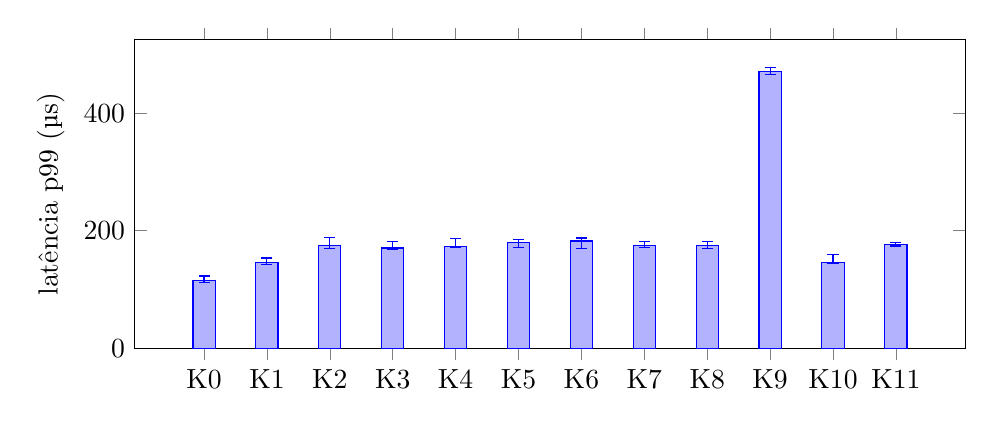
\begin{tikzpicture}
  \begin{axis}[width=\linewidth, height=5.5cm, ybar, bar width=8pt,
      ylabel={latência p99 (µs)}, xtick={0,...,11},
      xticklabels={K0,K1,K2,K3,K4,K5,K6,K7,K8,K9,K10,K11}, ymin=0,
      error bars/y dir=both, error bars/y explicit]
    \addplot+[error bars/.cd, y dir=both, y explicit] coordinates {
      (0,115.000) +- (0,0) -= (0,3.500) += (0,8.000)
      (1,146.500) +- (0,0) -= (0,4.500) += (0,7.000)
      (2,174.500) +- (0,0) -= (0,5.000) += (0,13.500)
      (3,170.500) +- (0,0) -= (0,2.000) += (0,11.500)
      (4,173.000) +- (0,0) -= (0,1.500) += (0,14.000)
      (5,179.500) +- (0,0) -= (0,8.500) += (0,5.500)
      (6,182.500) +- (0,0) -= (0,13.000) += (0,5.000)
      (7,174.500) +- (0,0) -= (0,3.000) += (0,7.000)
      (8,174.500) +- (0,0) -= (0,4.500) += (0,7.000)
      (9,470.000) +- (0,0) -= (0,4.000) += (0,7.000)
      (10,146.500) +- (0,0) -= (0,2.500) += (0,12.500)
      (11,176.000) +- (0,0) -= (0,2.000) += (0,4.500)
    };
  \end{axis}
\end{tikzpicture}
